%% Journal of Science and Medicine in Sport — Brief Report (anonymised manuscript)
%% Resubmission of JSAMS-D-26-02238 in the format the Editor-in-Chief suggested (03.11.2026).
%% Hand-condensed from the frozen ../manus/main.tex; every number is checked against it by kontroll_brief.py.
\documentclass[12pt,a4paper]{article}

\usepackage[utf8]{inputenc}
\usepackage[T1]{fontenc}
\usepackage{times}
\usepackage[margin=2.5cm]{geometry}
\usepackage{setspace}
\doublespacing

\usepackage{graphicx}
\graphicspath{{../figures/}}
\usepackage{float}
\usepackage{amsmath,amssymb}
\usepackage{booktabs}
\usepackage{caption}
\usepackage[colorlinks=true,linkcolor=blue,citecolor=blue,urlcolor=blue]{hyperref}
\usepackage[numbers,sort&compress]{natbib}
\usepackage{lineno}
\linenumbers

\begin{document}

\begin{center}
{\LARGE\bfseries Does starting age predict who stays? Competition debut and long-term participation in youth track and field\par}
\vspace{0.5em}
{\normalsize Anonymised manuscript (Brief Report)\par}
\end{center}

\section*{Abstract}

\noindent Whether early competitive entry harms or protects participation is contested. We followed 17\,496 athletes born 2001--2005 with a first registered competition at ages 10--16 in a national registry; 546 (3.1\,\%) became active seniors. Senior conversion was U-shaped with a null linear trend (OR 0.99 per year), but at equal career length later starters persisted less (OR 0.70 per year). Among athletes competing at 17, entry age added little once current competition volume was known (OR 0.85 to 0.99). Early entry carried no retention penalty; the first season after entry was the decisive filter.

\vspace{0.5em}
\noindent\textbf{Keywords:} Athletes$^\dagger$; Adolescent$^\dagger$; Child$^\dagger$; Registries$^\dagger$; Cohort studies$^\dagger$; attrition

\noindent{\footnotesize $^\dagger$Medical Subject Headings (MeSH) term.}

\newpage

\section{Introduction}

When should children enter competitive sport? Position statements on early specialisation caution that intensive training and competition at young ages risk overuse injury and burnout, the latter defined as ceasing to participate \cite{difiori2014}; on this reading, later entry should protect retention. The retention literature predicts the opposite: in a prospective study of 1\,762 Dutch football players, those who dropped out had started organised football later than those who stayed \cite{vanyperen2021}. Direct tests are scarce, and the retrospective expertise literature, which finds that world-class athletes started their main sport later than national-class peers \cite{barth2022,gullich2025}, samples on success. No study has followed a complete national entry population of an individual sport. The Norwegian athletics registry permits that design: every sanctioned result is registered, competition begins at age 10, and earlier studies of the registry found relative-age selection complete at entry \cite{guttormsen2026rae} and current competition volume a stronger predictor of senior retention than history (unpublished data). We asked whether debut age predicts senior activity (H1), whether later debutants exit faster on their own clock (H2), and whether entry history adds information beyond current engagement among athletes still competing at 17 (H3). The exposure is competition debut, not the start of sport participation.

\section{Methods}

We used a frozen extract of the Norwegian Athletics Federation's results database (29 October 2026); only participation fields were extracted, and no performance data were used at any age. Age is calendar-year age. Of 28\,339 athletes with an approved result at age 10 or older, the primary sample comprises the 17\,496 born 2001--2005 whose first approved result fell at ages 10--16, cohorts followed past age 20 for everyone (50.1\,\% female; sample flow in Supplementary Table S1, characteristics in Table S6). Debut age was treated categorically (reference 10) and as a linear trend. The primary outcome, active senior, is at least two approved results in the same calendar year at age 20 or older. Because later entrants have fewer seasons to cover before a fixed age, a second outcome measured persistence at equal career length: at least two competition days in a single season four or more years after the debut season (five and six years as sensitivity), among athletes for whom that season was observable by 2025. Retention $k$ years after debut ($k$ = 1--5) was the share with a result in the calendar year debut + $k$, with per-$k$ denominators. H1 and the equal-career-length outcome were estimated by logistic regression adjusted for sex, birth cohort and club size, with a likelihood-ratio test of the categorical against the linear coding. H3 was a landmark analysis \cite{anderson1983} among athletes with an approved result in the age-17 season itself, regressing senior activity on debut age with sex and cohort, with and without competition days at ages 16--17. Pre-specified robustness analyses excluded COVID-19 debuts (2020--2021), varied the outcome, added debut-season volume and split the cohorts (Table S5). The analysis plan was committed to version control before any exposure--outcome model was estimated; reporting follows STROBE \cite{vonelm2007}. The study is not health research under Norway's Health Research Act, Sikt confirmed that the data use raises no data-protection concerns, and no individual is identified.

\section{Results}

Debut at 10 was the most common entry point, rising from 32.6\,\% of debutants born 2001 to 43.9\,\% of those born 2008, and roughly one debutant in six entered at 14 or later (Figure S1). The median debutant competed on a single day in the debut season, at every entry age.

Of the 17\,496 debutants, 546 (3.1\,\%) were active as seniors. Conversion was U-shaped (Table~\ref{tab:h1}; Figure S2): 3.8\,\% for debut at 10, lower at every age from 11 to 14 and higher again at 15 and 16; a likelihood-ratio test rejected the linear coding (LR = 43.2, df = 5, p = 3.3 $\times$ 10$^{-8}$). Adjusted odds were significantly lower for debuts at 11, 12 and 14 (OR 0.53--0.63), directionally lower at 13 (OR 0.75, 95\,\% CI 0.55--1.02), equal at 15 (OR 1.00) and higher at 16 (OR 1.73, 95\,\% CI 1.15--2.59, resting on 28 events); the linear trend was null (OR 0.99 per year, 95\,\% CI 0.94--1.04). The elevation at 16 rests on the COVID-19 seasons: all 107 debut-16 athletes born 2004--2005 debuted in 2020 or 2021, and excluding those debuts or adding a COVID-19 flag left the debut-16 estimate non-significant while the odds at 11--14 were unchanged (Table S5). Conversion was higher for boys than girls at every debut age, with the same U in both sexes (Table S2).

\begin{table}[H]
\centering
\caption{Senior activity (age $\geq$20) and competing at equal career length, by debut age (n = 17\,496; 546 senior events, 2\,312 equal-career-length events). \% = raw proportion; odds ratios relative to debut at age 10, adjusted for sex, birth cohort, and club size. Competing $\geq$4 years after debut: at least two competition days in a single season four or more years after the debut season. A likelihood-ratio test favours the categorical over the linear coding for the senior outcome (LR = 43.2, df = 5, p $<$ 0.001); the debut-16 senior estimate rests on 28 events and is not robust to excluding debuts in 2020--2021 (Supplementary Table S5). Abbreviations: CI, confidence interval; LR, likelihood ratio; OR, odds ratio.}
\label{tab:h1}
\small
\begin{tabular}{lrcccc}
\toprule
 & & \multicolumn{2}{c}{Active senior (age $\geq$20)} & \multicolumn{2}{c}{Competing $\geq$4 years after debut} \\
\cmidrule(lr){3-4}\cmidrule(lr){5-6}
Debut age & n & \% & OR (95\,\% CI) & \% & OR (95\,\% CI) \\
\midrule
10 & 6\,626 & 3.8 & 1.00 (ref.) & 20.4 & 1.00 (ref.) \\
11 & 3\,616 & 2.4 & 0.63 (0.49--0.81) & 12.4 & 0.56 (0.50--0.63) \\
12 & 2\,529 & 2.1 & 0.53 (0.39--0.71) & 8.5 & 0.37 (0.31--0.43) \\
13 & 1\,691 & 2.9 & 0.75 (0.55--1.02) & 8.7 & 0.37 (0.31--0.44) \\
14 & 1\,747 & 2.4 & 0.62 (0.44--0.86) & 4.5 & 0.19 (0.15--0.24) \\
15 & 863 & 3.9 & 1.00 (0.70--1.45) & 4.9 & 0.21 (0.15--0.29) \\
16 & 424 & 6.6 & 1.73 (1.15--2.59) & 6.6 & 0.29 (0.20--0.43) \\
\midrule
Linear trend, per +1 year &  &  & 0.99 (0.94--1.04) &  & 0.70 (0.68--0.72) \\
\bottomrule
\end{tabular}

\end{table}

Aligned on time since debut (Figure~\ref{fig:retk}; Table S3), early entrants were far more durable: one year after the debut season, 51\,\% of those who debuted at 10 were still competing, against 26--40\,\% of those who debuted at 11--16, and after five years 17\,\% against 3--10\,\%. At equal career length, 20.4\,\% of those who debuted at 10 competed on at least two days in a season four or more years later, against 4.5--6.6\,\% of those who debuted at 14--16, an adjusted OR of 0.70 per year of later debut (95\,\% CI 0.68--0.72), essentially unchanged at five and six years (Table S4). The decline was concentrated between debut at 10 and 14 and did not continue beyond 14. On the age clock, the debut groups were within about a percentage point of one another at ages 20 and 21 (Figure S3).

\begin{figure}[H]
\centering
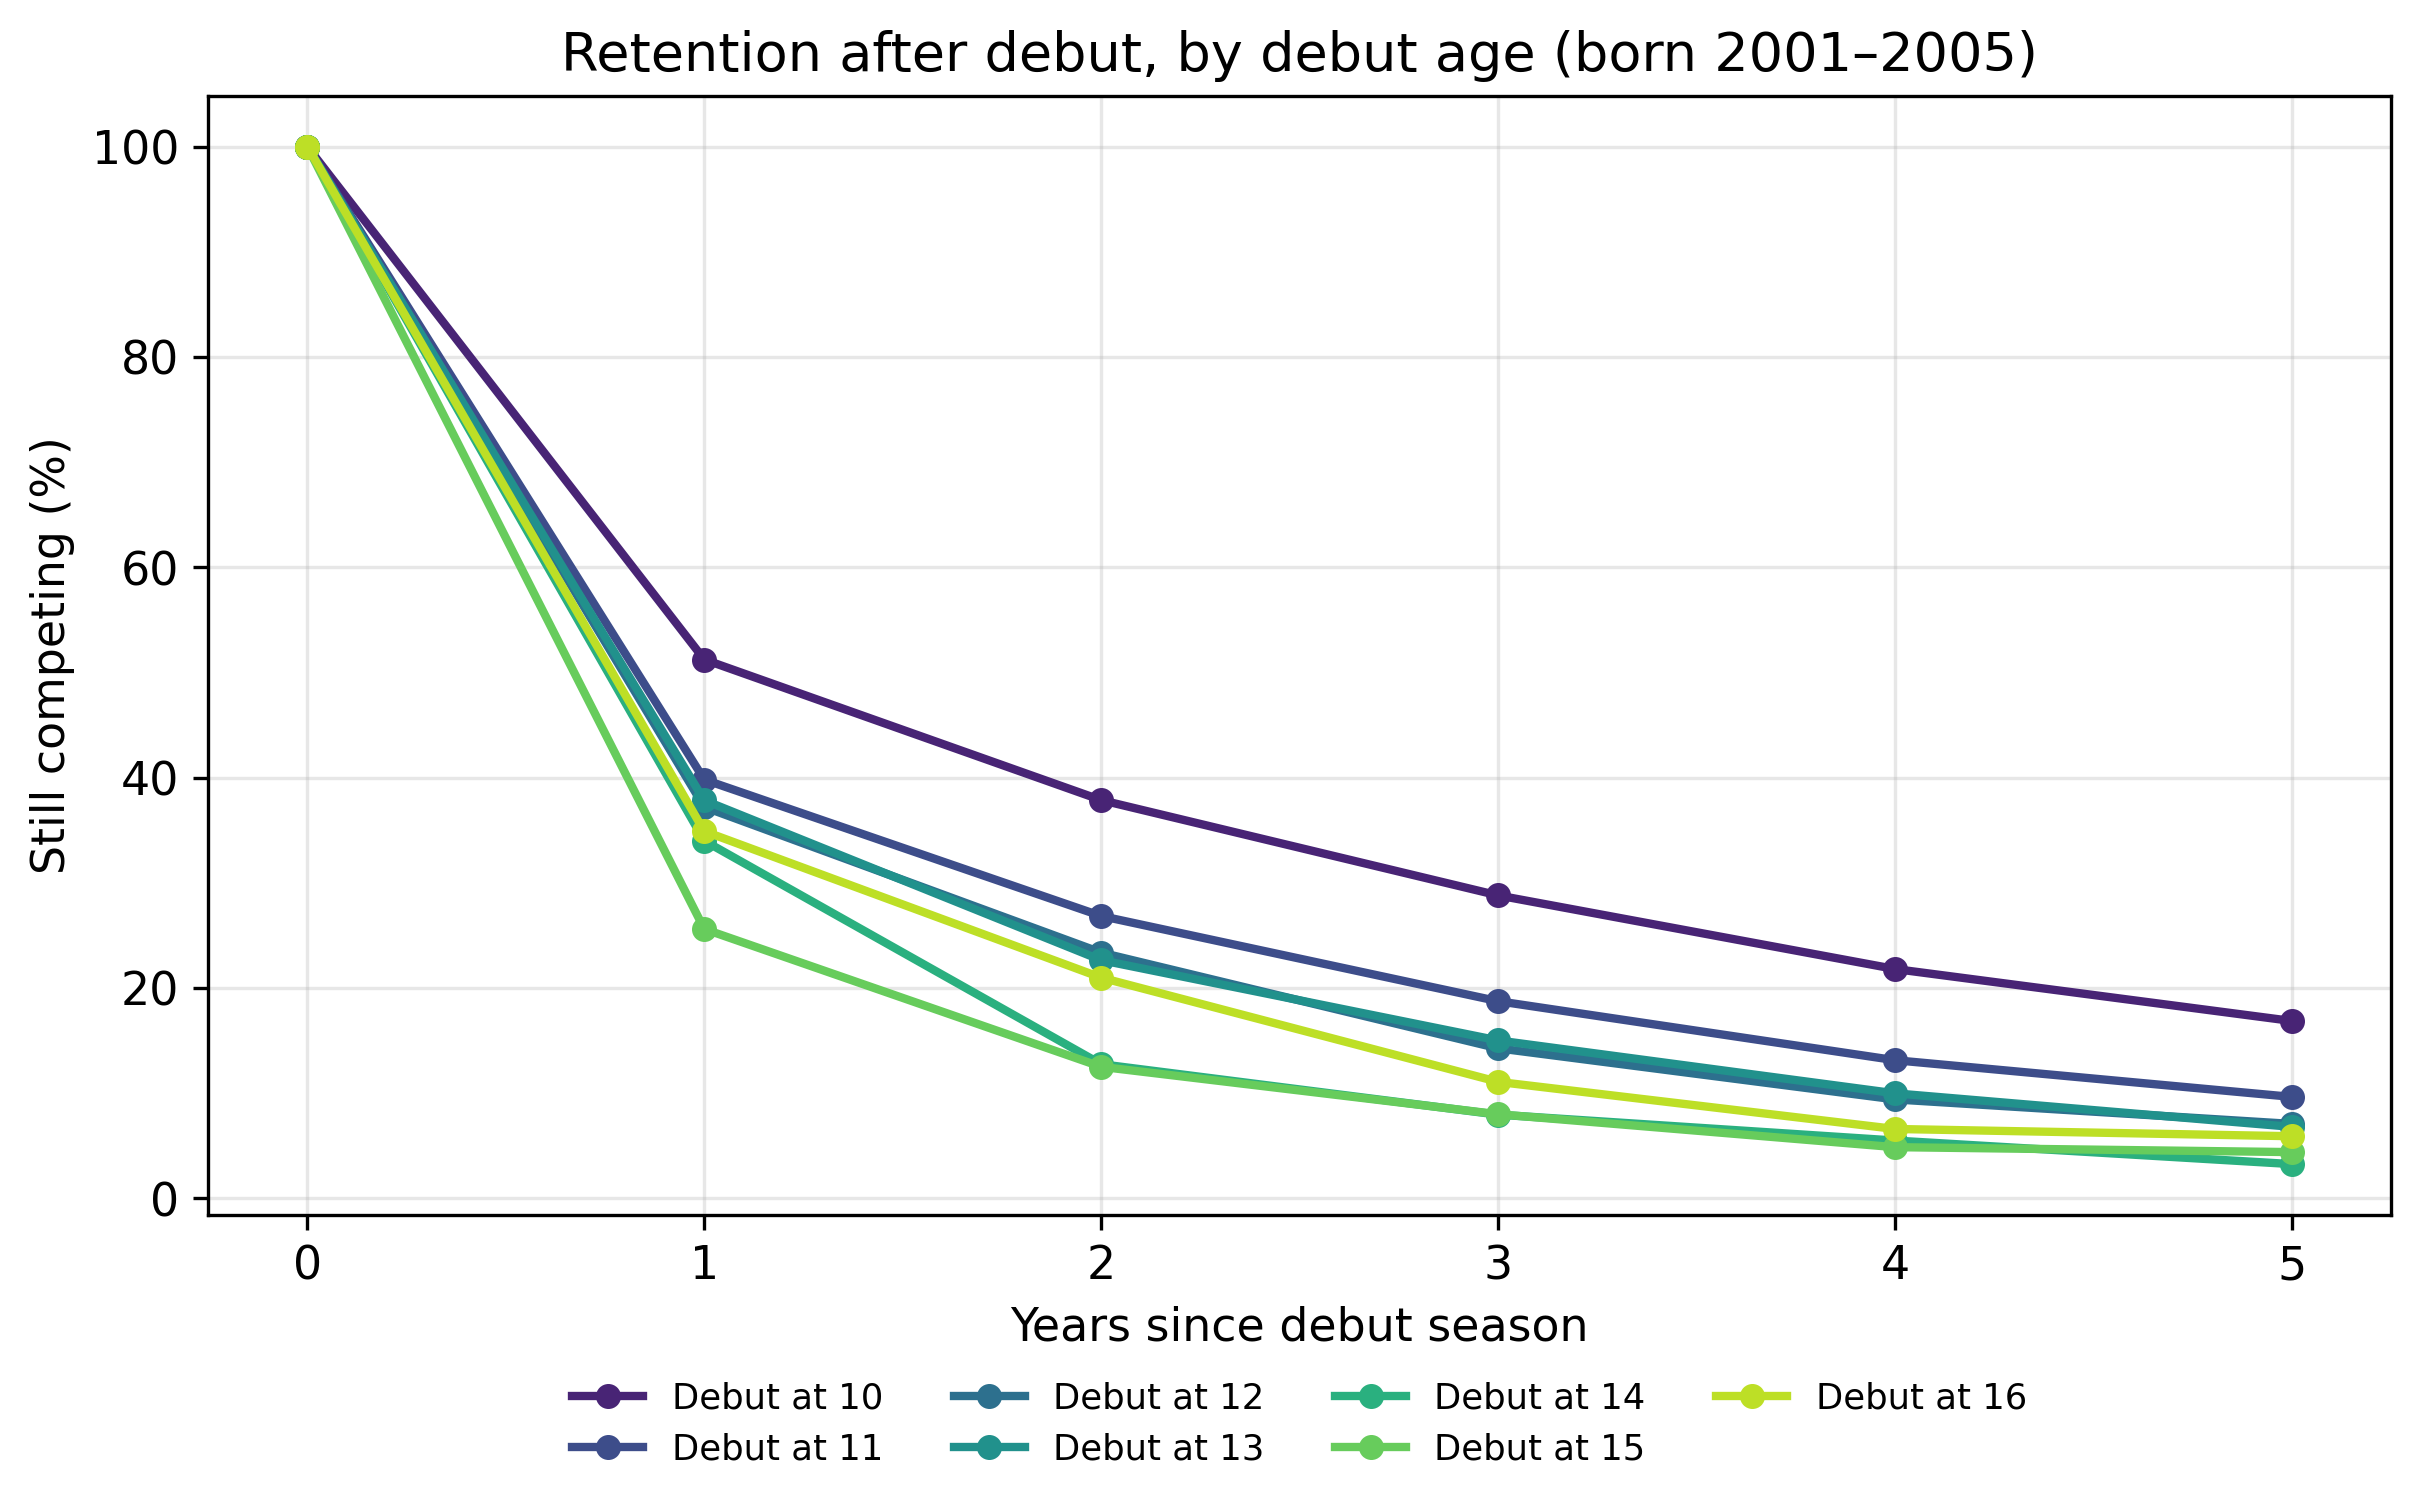
\includegraphics[width=0.85\textwidth]{fig3_retention_k.png}
\caption{Retention $k$ years after the debut season (at least one approved result in the calendar year debut + $k$), by debut age (born 2001--2005; athlete-years fully observable by 2025). Wilson 95\,\% intervals for every cell are given in Supplementary Table S3.}
\label{fig:retk}
\end{figure}

Of the 17\,496 debutants, 1\,637 (9.4\,\%) competed in the age-17 season itself, and 472 of these (28.8\,\%) became active seniors. In this landmark sample, earlier debut appeared advantageous (OR 0.85 per year of later debut, 95\,\% CI 0.80--0.90), but adding competition days at ages 16--17 brought the association close to null (OR 0.99, 95\,\% CI 0.92--1.05). None of the robustness variants moved the linear trend far from null (odds ratios 0.94 to 1.00 per year; Table S5).

\section{Discussion}

In the complete entry population of Norwegian youth track and field, age at first competition carried no simple message about who would still be competing as an adult. At a fixed adult age the association was U-shaped with a null trend; measured from each athlete's own start, later entrants left much faster. The fixed-age U is the sum of these faster exits and the shorter distance late entrants have to the outcome age. Neither of the positions that motivated the study was formulated about this exposure: the specialisation cautions concern intensive, year-round involvement \cite{difiori2014}, not whether a ten-year-old appears once in a sanctioned meet, and the football finding concerns joining organised sport \cite{vanyperen2021}, whereas a late debutant here may have trained for years before a first meet. On the margin the registry can test, early entry carried no retention penalty, and later entrants persisted less at equal career length, as the football study found for later joiners. Both arms of the U plausibly reflect selection, and the entire U may be compositional.

The dominant feature of every debut group is the first-year cliff: between half and three quarters of each entry cohort did not compete in the season after debut, so most of whatever determines long-term engagement acts within a season or two of arrival. Among athletes competing at 17, entry history added little once current volume was known, repeating what the registry has shown for early volume and early progression (unpublished data). The claim is predictive: current volume is plausibly a mediator of entry timing, and the landmark conditions on survival. Competition debut is not sport start, exit from the registry is not exit from sport, selection into debut age is unmeasured, birth dates are missing for most brief early participants, and coverage in 2011, the first electronic season, is thinner than in later years; no causal reading is offered.

\section{Conclusion}

Early competitive entry did not undermine retention: per year of career, early entrants persisted longest, and every entry age from 10 to 19 produced senior athletes. Retention effort is better aimed at the first seasons after entry than at the timing of entry, and by late adolescence current engagement says more than entry history.

\section*{Acknowledgments}

\noindent The author thanks the Norwegian Athletics Federation, whose systematic registration of competition results makes population research of this kind possible. This research did not receive any specific grant from funding agencies in the public, commercial, or not-for-profit sectors. Declarations of interest: none; the author maintains an open, non-commercial statistics platform built on the federation's public results database.

\section*{Data availability}

\noindent The competition records are publicly accessible via the Norwegian Athletics Federation's online register for ages 13 and above; records for the 10--12 age classes are not publicly released. The derived dataset contains personal data (dates of birth) and cannot be shared; the analysis code will be deposited in a public repository upon acceptance. Supplementary Tables S1--S6 and Figures S1--S3 accompany the submission.

\section*{Declaration of generative AI and AI-assisted technologies in the writing process}

\noindent During the preparation of this work the author used Anthropic Claude (Claude Opus 5.5) in order to improve language and readability, assist with structuring the text, check analysis code and identify errors. After using this tool, the author reviewed and edited the content as needed and takes full responsibility for the content of the publication.

\bibliographystyle{../manus_jsams/jsams}
\bibliography{../manus_jsams/references}

\end{document}
